% Seminar 4: Probability
% Statistics of Financial Markets -- Bachelor's programme, Bucharest University of Economic Studies
% GENERATED by latex/build_seminar4.py -- edit the generator, not this file.
% Student version by default; the instructor version is the *_solutions.tex wrapper.
\makeatletter\@ifundefined{ifsolutions}{\expandafter\newif\csname ifsolutions\endcsname}{}\makeatother

\newcommand{\coursename}{Statistics of Financial Markets}
% Preambul comun SFM -- Statistica piețelor financiare / Statistics of Financial Markets (Beamer, 16:9)
% Același design ca MFM. Înainte de % Preambul comun SFM -- Statistica piețelor financiare / Statistics of Financial Markets (Beamer, 16:9)
% Același design ca MFM. Înainte de % Preambul comun SFM -- Statistica piețelor financiare / Statistics of Financial Markets (Beamer, 16:9)
% Același design ca MFM. Înainte de \input{../../latex/preamble} se definește
%   \newcommand{\coursename}{Statistics of Financial Markets}      (EN)
%   \newcommand{\coursename}{Statistica piețelor financiare}       (RO)  și  \def\sfmlang{ro}
% Fișierele .tex se află în EN/Courses, EN/Seminars, RO/Cursuri, RO/Seminarii (două niveluri sub rădăcină).
% Deck-urile sînt generate de latex/build_chapterN.py / build_seminarN.py (vezi latex/sfm_build.py).

\documentclass[9pt, aspectratio=169, t]{beamer}
\providecommand{\coursename}{Statistics of Financial Markets}

% Ensure content fits on slides
\setbeamersize{text margin left=8mm, text margin right=8mm}

%=============================================================================
% THEME AND STYLE CONFIGURATION
%=============================================================================
\usetheme{default}
% Using default theme for clean header/footer control

% Color Palette (matching Redispatch PDF)
\definecolor{MainBlue}{RGB}{26, 58, 110}
\definecolor{AccentBlue}{RGB}{26, 58, 110}
\definecolor{IDAred}{RGB}{205, 0, 0}
\definecolor{DarkGray}{RGB}{51, 51, 51}
\definecolor{MediumGray}{RGB}{128, 128, 128}
\definecolor{LightGray}{RGB}{248, 248, 248}
\definecolor{VeryLightGray}{RGB}{235, 235, 235}
\definecolor{KeynoteGray}{RGB}{218, 218, 218}
\definecolor{SectionGray}{RGB}{120, 120, 120}
\definecolor{FooterGray}{RGB}{100, 100, 100}
\definecolor{Crimson}{RGB}{220, 53, 69}
\definecolor{Forest}{RGB}{46, 125, 50}
\definecolor{Amber}{RGB}{181, 133, 63}
\definecolor{Orange}{RGB}{230, 126, 34}
\definecolor{Purple}{RGB}{142, 68, 173}

% Gradient background (exact Keynote 315° gradient: white to RGB 218,218,218)
\setbeamertemplate{background}{%
    \begin{tikzpicture}[remember picture, overlay]
        \shade[shading=axis, shading angle=315,
        top color=white, bottom color=KeynoteGray]
        (current page.south west) rectangle (current page.north east);
    \end{tikzpicture}%
}
% Fallback solid color for compatibility
\setbeamercolor{background canvas}{bg=}

\setbeamercolor{palette primary}{bg=MainBlue, fg=white}
\setbeamercolor{palette secondary}{bg=MainBlue!85, fg=white}
\setbeamercolor{palette tertiary}{bg=MainBlue!70, fg=white}
\setbeamercolor{structure}{fg=MainBlue}
\setbeamercolor{title}{fg=IDAred}
\setbeamercolor{frametitle}{fg=IDAred, bg=}
\setbeamercolor{block title}{bg=MainBlue, fg=white}
\setbeamercolor{block body}{bg=VeryLightGray, fg=DarkGray}
\setbeamercolor{block title alerted}{bg=Crimson, fg=white}
\setbeamercolor{block body alerted}{bg=Crimson!8, fg=DarkGray}
\setbeamercolor{block title example}{bg=Forest, fg=white}
\setbeamercolor{block body example}{bg=Forest!8, fg=DarkGray}
\setbeamercolor{item}{fg=MainBlue}

% Footer colors (override Madrid theme blue)
\setbeamercolor{author in head/foot}{fg=FooterGray, bg=}
\setbeamercolor{title in head/foot}{fg=FooterGray, bg=}
\setbeamercolor{date in head/foot}{fg=FooterGray, bg=}
\setbeamercolor{section in head/foot}{fg=FooterGray, bg=}
\setbeamercolor{subsection in head/foot}{fg=FooterGray, bg=}

% Bullet styles (apply everywhere including blocks)
\setbeamertemplate{itemize item}{\color{MainBlue}$\boxdot$}
\setbeamertemplate{itemize subitem}{\color{MainBlue}$\blacktriangleright$}
\setbeamertemplate{itemize subsubitem}{\color{MainBlue}\tiny$\bullet$}
\setbeamertemplate{itemize/enumerate body begin}{\normalsize}
\setbeamertemplate{itemize/enumerate subbody begin}{\normalsize}

% Item spacing - compact style
\setlength{\leftmargini}{10pt}       % Level 1: minimal indent
\setlength{\leftmarginii}{10pt}      % Level 2: minimal additional indent
% Compact list spacing (zero extra space before/after lists in blocks)
\makeatletter
\def\@listi{\leftmargin\leftmargini \topsep 0pt \parsep 0pt \itemsep 0pt}
\def\@listii{\leftmargin\leftmarginii \topsep 0pt \parsep 0pt \itemsep 0pt}
\makeatother

\setbeamertemplate{navigation symbols}{}

%=============================================================================
% CUSTOM HEADLINE
%=============================================================================
\setbeamertemplate{headline}{%
    \vskip10pt%
    \hbox to \paperwidth{%
        \hskip0.5cm%
        {\small\color{FooterGray}\renewcommand{\hyperlink}[2]{##2}\insertsectionhead}%
        \hfill%
        \textcolor{FooterGray}{\small\insertframenumber}%
        \hskip0.5cm%
    }%
    \vskip4pt%
    {\color{FooterGray}\hrule height 0.4pt}%
}

%=============================================================================
% CUSTOM FOOTER
%=============================================================================
\usepackage{fontawesome5}

\setbeamertemplate{footline}{%
    {\color{FooterGray}\hrule height 0.4pt}%
    \vskip4pt%
    \hbox to \paperwidth{%
        \hskip0.5cm%
        \textcolor{FooterGray}{\small\coursename}%
        \hfill%
        \raisebox{-0.1em}{%
            \begin{tikzpicture}[x=0.08em, y=0.08em, line width=0.4pt]
                \draw[FooterGray] (0,3) -- (1,4) -- (2,3.5) -- (3,5) -- (4,4) -- (5,6) -- (6,5.5) -- (7,4) -- (8,5) -- (9,7) -- (10,6) -- (11,5) -- (12,6.5) -- (13,8) -- (14,7) -- (15,6) -- (16,7.5) -- (17,9) -- (18,8) -- (19,7) -- (20,8.5) -- (21,10) -- (22,9) -- (23,8) -- (24,9.5);
            \end{tikzpicture}%
        }%
        \hskip0.5cm%
    }%
    \vskip6pt%
}

%=============================================================================
% PACKAGES
%=============================================================================
\usepackage[utf8]{inputenc}
\DeclareUnicodeCharacter{03B1}{\ensuremath{\alpha}}
\usepackage[T1]{fontenc}
\usepackage{amsmath, amssymb, amsthm}
\usepackage{mathtools}
\usepackage{bm}
\usepackage{tikz}
\usetikzlibrary{arrows.meta, positioning, shapes, calc, decorations.pathreplacing, shadings}
\usepackage{booktabs}
\usepackage{multirow}
\usepackage{array}
\usepackage{graphicx}
\usepackage{hyperref}
\usepackage{colortbl}
\usepackage{listings}
\lstset{language=Python, basicstyle=\ttfamily\scriptsize, keywordstyle=\color{MainBlue}\bfseries,
  commentstyle=\color{Forest}, stringstyle=\color{Crimson}, breaklines=true,
  frame=none, backgroundcolor=\color{VeryLightGray}, xleftmargin=2mm}
\hypersetup{colorlinks=true, linkcolor=MainBlue, urlcolor=MainBlue}
\graphicspath{{../../logos/}{../../charts/}{../../photos/}}
\usepackage{xcolor}
\hfuzz=2pt  % Suppress tiny overfull warnings (<2pt)
\vfuzz=2pt  % Suppress tiny vertical overfull warnings (<2pt)

%=============================================================================
% QUANTLET COMMANDS
%   \quantlet{<displayed name>}{<url>}       (generic, compatible with the older SFM decks)
%   \sfmquantlet{Ch_05}{SFM_ch5_garch}       -> https://github.com/danpele/SFM/tree/main/Quantlets/Ch_05/SFM_ch5_garch
%   \qlurl{<folder>} is defined per chapter by the generator (Quantlets/Ch_NN/<folder>)
%=============================================================================
\newcommand{\sfmrepo}{https://github.com/danpele/SFM}
\newcommand{\sfmqlbase}{https://github.com/danpele/SFM/tree/main/Quantlets}
\newcommand{\quantlet}[2]{%
    \hfill\href{#2}{%
        \raisebox{-0.15em}{
\includegraphics[height=0.7em]{ql_logo.png}}%
        \textcolor{MainBlue}{\tiny\ #1}%
    }%
}
\newcommand{\sfmquantlet}[2]{\quantlet{\detokenize{#2}}{\sfmqlbase/#1/#2}}

%=============================================================================
% NOTEBOOKS (Google Colab)
%   \colaburl{notebooks/EN/chapter5_seminar_notebook.ipynb} -> the Colab link of a file in the SFM repo
%   \nb: the chapter notebook (each seminar deck redefines it with \renewcommand)
%=============================================================================
\newcommand{\colaburl}[1]{https://colab.research.google.com/github/danpele/SFM/blob/main/#1}
\newcommand{\nb}{https://colab.research.google.com/github/danpele/SFM/tree/main/notebooks/EN}
\newcommand{\nbname}{notebooks/EN}

%=============================================================================
% SLIDE HELPERS (used by the generators; the same as in MFM)
%=============================================================================
% local font size for list bodies (the preamble forces \normalsize)
\newcommand{\itemsize}[1]{\setbeamertemplate{itemize/enumerate body begin}{#1}\setbeamertemplate{itemize/enumerate subbody begin}{#1}}
\newcommand{\intitle}[1]{{\hypersetup{urlcolor=white}#1}}   % white links inside coloured title bars
\newcommand{\imgcap}[1]{{\scriptsize #1}\\[0.5mm]}          % caption under a photo
\newcommand{\imgcredit}[2]{{\tiny\color{FooterGray}\href{#1}{#2}}}   % image credit: source URL, author/licence
\newcommand{\aiprompt}[1]{{\ttfamily\color{MainBlue}#1}}     % a prompt to an AI assistant

%=============================================================================
% SEMINARS: student version by default; the instructor wrapper *_solutions.tex sets \solutionstrue
%=============================================================================
\makeatletter\@ifundefined{ifsolutions}{\expandafter\newif\csname ifsolutions\endcsname}{}\makeatother
\newcommand{\solonly}[1]{\ifsolutions #1\fi}
\newcommand{\propsub}{\ifsolutions\else\framesubtitle{\ifdefined\sfmlang Rezolvarea se discută la seminar\else Solution discussed in class\fi}\fi}

%=============================================================================
% APPENDIX AND CHAPTER LINKS (latex/appendix_links.py writes the calls; it also re-declares these
% macros before \begin{document}, so the decks compile with or without this preamble block)
%=============================================================================
\providecommand{\sfmapplink}[3]{\hypertarget{#2}{}\hyperlink{#1}{\beamergotobutton{#3}}}
\providecommand{\sfmappback}[2]{\begin{tikzpicture}[remember picture,overlay]\node[anchor=south east] at ([xshift=-3mm,yshift=7mm]current page.south east){\hyperlink{#1}{\beamerreturnbutton{#2}}};\end{tikzpicture}}
\providecommand{\sfmchlink}[2]{\href{#1}{#2}}
\providecommand{\sfmchlinkt}[2]{\href{#1}{\usebeamercolor[fg]{frametitle}#2}}

%=============================================================================
% QUANTINAR COMMAND: link către un curs Quantinar (subiecte avansate)
%=============================================================================
\newcommand{\quantinar}[2]{%
    \href{#2}{%
        \raisebox{-0.15em}{
\includegraphics[height=0.8em]{qr_logo.png}}%
        \textcolor{MainBlue}{\scriptsize\ #1}%
    }%
}

%=============================================================================
% CUSTOM TITLE PAGE
%=============================================================================
\defbeamertemplate*{title page}{hybrid}[1][]
{
    \vspace{0.2cm}
    % Logos row - top header (with clickable links)
    \begin{center}
        \href{https://www.ase.ro}{
\includegraphics[height=1.0cm]{ase_logo.png}}\hspace{0.3cm}%
        \href{https://theida.net}{
\includegraphics[height=1.0cm]{ida_logo.png}}\hspace{0.3cm}%
        \href{https://blockchain-research-center.com}{
\includegraphics[height=1.0cm]{brc_logo.png}}\hspace{0.3cm}%
        \href{https://www.ai4efin.ase.ro}{
\includegraphics[height=1.0cm]{ai4efin_logo.png}}\hspace{0.3cm}%
        \href{https://ipe.ro/new}{
\includegraphics[height=1.0cm]{acad_logo.png}}\hspace{0.3cm}%
        \href{https://www.digital-finance-msca.com}{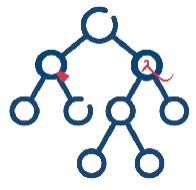
\includegraphics[height=1.0cm]{msca_logo.png}}%
    \end{center}

    \vspace{0.6cm}

    % Main title with Q logos on sides (with clickable links)
    \begin{center}
        \begin{minipage}{0.1\textwidth}
            \centering
            \href{https://quantlet.com}{
\includegraphics[height=1.1cm]{ql_logo.png}}
        \end{minipage}%
        \begin{minipage}{0.78\textwidth}
            \centering
            {\LARGE\bfseries\usebeamercolor[fg]{title}\inserttitle}

            \vspace{0.3cm}

            {\usebeamerfont{subtitle}\usebeamercolor[fg]{title}\insertsubtitle}
        \end{minipage}%
        \begin{minipage}{0.1\textwidth}
            \centering
            \href{https://quantinar.com}{
\includegraphics[height=1.1cm]{qr_logo.png}}
        \end{minipage}
    \end{center}

    \vspace{0.6cm}

    % Authors (left aligned)
    \hspace{0.5cm}{\usebeamerfont{author}\insertauthor}

    \vspace{0.3cm}

    % Institute/Affiliations (left aligned)
    \hspace{0.5cm}\begin{minipage}[t]{0.9\textwidth}
        \raggedright\small\insertinstitute
    \end{minipage}
}

%=============================================================================
% THEOREM ENVIRONMENTS
%=============================================================================
\theoremstyle{definition}
\setbeamertemplate{theorems}[numbered]
\ifdefined\sfmlang
\newtheorem{defn}{Definiție}
\newtheorem{thm}{Teoremă}
\newtheorem{prop}{Propoziție}
\newtheorem{rmk}{Observație}
\else
\newtheorem{defn}{Definition}
\newtheorem{thm}{Theorem}
\newtheorem{prop}{Proposition}
\newtheorem{rmk}{Remark}
\fi

%=============================================================================
% CENTRED MINIPAGE (no extra vertical space)
%=============================================================================
\newenvironment{cminipage}[1]{%
    \par\noindent\hfill\begin{minipage}{#1}\ignorespaces
}{%
    \end{minipage}\hfill\null\par
}

%=============================================================================
% CUSTOM COMMANDS
%=============================================================================
\newcommand{\E}{\mathbb{E}}
\newcommand{\Var}{\text{Var}}
\newcommand{\Cov}{\text{Cov}}
\newcommand{\Corr}{\text{Corr}}
\newcommand{\R}{\mathbb{R}}
\newcommand{\N}{\mathbb{N}}
\newcommand{\Z}{\mathbb{Z}}
\newcommand{\B}{\mathbf{B}}
\newcommand{\imark}{\textcolor{MainBlue}{\textbullet}}
\newcommand{\RMSE}{\text{RMSE}}
\newcommand{\MAE}{\text{MAE}}
\newcommand{\MAPE}{\text{MAPE}}

 se definește
%   \newcommand{\coursename}{Statistics of Financial Markets}      (EN)
%   \newcommand{\coursename}{Statistica piețelor financiare}       (RO)  și  \def\sfmlang{ro}
% Fișierele .tex se află în EN/Courses, EN/Seminars, RO/Cursuri, RO/Seminarii (două niveluri sub rădăcină).
% Deck-urile sînt generate de latex/build_chapterN.py / build_seminarN.py (vezi latex/sfm_build.py).

\documentclass[9pt, aspectratio=169, t]{beamer}
\providecommand{\coursename}{Statistics of Financial Markets}

% Ensure content fits on slides
\setbeamersize{text margin left=8mm, text margin right=8mm}

%=============================================================================
% THEME AND STYLE CONFIGURATION
%=============================================================================
\usetheme{default}
% Using default theme for clean header/footer control

% Color Palette (matching Redispatch PDF)
\definecolor{MainBlue}{RGB}{26, 58, 110}
\definecolor{AccentBlue}{RGB}{26, 58, 110}
\definecolor{IDAred}{RGB}{205, 0, 0}
\definecolor{DarkGray}{RGB}{51, 51, 51}
\definecolor{MediumGray}{RGB}{128, 128, 128}
\definecolor{LightGray}{RGB}{248, 248, 248}
\definecolor{VeryLightGray}{RGB}{235, 235, 235}
\definecolor{KeynoteGray}{RGB}{218, 218, 218}
\definecolor{SectionGray}{RGB}{120, 120, 120}
\definecolor{FooterGray}{RGB}{100, 100, 100}
\definecolor{Crimson}{RGB}{220, 53, 69}
\definecolor{Forest}{RGB}{46, 125, 50}
\definecolor{Amber}{RGB}{181, 133, 63}
\definecolor{Orange}{RGB}{230, 126, 34}
\definecolor{Purple}{RGB}{142, 68, 173}

% Gradient background (exact Keynote 315° gradient: white to RGB 218,218,218)
\setbeamertemplate{background}{%
    \begin{tikzpicture}[remember picture, overlay]
        \shade[shading=axis, shading angle=315,
        top color=white, bottom color=KeynoteGray]
        (current page.south west) rectangle (current page.north east);
    \end{tikzpicture}%
}
% Fallback solid color for compatibility
\setbeamercolor{background canvas}{bg=}

\setbeamercolor{palette primary}{bg=MainBlue, fg=white}
\setbeamercolor{palette secondary}{bg=MainBlue!85, fg=white}
\setbeamercolor{palette tertiary}{bg=MainBlue!70, fg=white}
\setbeamercolor{structure}{fg=MainBlue}
\setbeamercolor{title}{fg=IDAred}
\setbeamercolor{frametitle}{fg=IDAred, bg=}
\setbeamercolor{block title}{bg=MainBlue, fg=white}
\setbeamercolor{block body}{bg=VeryLightGray, fg=DarkGray}
\setbeamercolor{block title alerted}{bg=Crimson, fg=white}
\setbeamercolor{block body alerted}{bg=Crimson!8, fg=DarkGray}
\setbeamercolor{block title example}{bg=Forest, fg=white}
\setbeamercolor{block body example}{bg=Forest!8, fg=DarkGray}
\setbeamercolor{item}{fg=MainBlue}

% Footer colors (override Madrid theme blue)
\setbeamercolor{author in head/foot}{fg=FooterGray, bg=}
\setbeamercolor{title in head/foot}{fg=FooterGray, bg=}
\setbeamercolor{date in head/foot}{fg=FooterGray, bg=}
\setbeamercolor{section in head/foot}{fg=FooterGray, bg=}
\setbeamercolor{subsection in head/foot}{fg=FooterGray, bg=}

% Bullet styles (apply everywhere including blocks)
\setbeamertemplate{itemize item}{\color{MainBlue}$\boxdot$}
\setbeamertemplate{itemize subitem}{\color{MainBlue}$\blacktriangleright$}
\setbeamertemplate{itemize subsubitem}{\color{MainBlue}\tiny$\bullet$}
\setbeamertemplate{itemize/enumerate body begin}{\normalsize}
\setbeamertemplate{itemize/enumerate subbody begin}{\normalsize}

% Item spacing - compact style
\setlength{\leftmargini}{10pt}       % Level 1: minimal indent
\setlength{\leftmarginii}{10pt}      % Level 2: minimal additional indent
% Compact list spacing (zero extra space before/after lists in blocks)
\makeatletter
\def\@listi{\leftmargin\leftmargini \topsep 0pt \parsep 0pt \itemsep 0pt}
\def\@listii{\leftmargin\leftmarginii \topsep 0pt \parsep 0pt \itemsep 0pt}
\makeatother

\setbeamertemplate{navigation symbols}{}

%=============================================================================
% CUSTOM HEADLINE
%=============================================================================
\setbeamertemplate{headline}{%
    \vskip10pt%
    \hbox to \paperwidth{%
        \hskip0.5cm%
        {\small\color{FooterGray}\renewcommand{\hyperlink}[2]{##2}\insertsectionhead}%
        \hfill%
        \textcolor{FooterGray}{\small\insertframenumber}%
        \hskip0.5cm%
    }%
    \vskip4pt%
    {\color{FooterGray}\hrule height 0.4pt}%
}

%=============================================================================
% CUSTOM FOOTER
%=============================================================================
\usepackage{fontawesome5}

\setbeamertemplate{footline}{%
    {\color{FooterGray}\hrule height 0.4pt}%
    \vskip4pt%
    \hbox to \paperwidth{%
        \hskip0.5cm%
        \textcolor{FooterGray}{\small\coursename}%
        \hfill%
        \raisebox{-0.1em}{%
            \begin{tikzpicture}[x=0.08em, y=0.08em, line width=0.4pt]
                \draw[FooterGray] (0,3) -- (1,4) -- (2,3.5) -- (3,5) -- (4,4) -- (5,6) -- (6,5.5) -- (7,4) -- (8,5) -- (9,7) -- (10,6) -- (11,5) -- (12,6.5) -- (13,8) -- (14,7) -- (15,6) -- (16,7.5) -- (17,9) -- (18,8) -- (19,7) -- (20,8.5) -- (21,10) -- (22,9) -- (23,8) -- (24,9.5);
            \end{tikzpicture}%
        }%
        \hskip0.5cm%
    }%
    \vskip6pt%
}

%=============================================================================
% PACKAGES
%=============================================================================
\usepackage[utf8]{inputenc}
\DeclareUnicodeCharacter{03B1}{\ensuremath{\alpha}}
\usepackage[T1]{fontenc}
\usepackage{amsmath, amssymb, amsthm}
\usepackage{mathtools}
\usepackage{bm}
\usepackage{tikz}
\usetikzlibrary{arrows.meta, positioning, shapes, calc, decorations.pathreplacing, shadings}
\usepackage{booktabs}
\usepackage{multirow}
\usepackage{array}
\usepackage{graphicx}
\usepackage{hyperref}
\usepackage{colortbl}
\usepackage{listings}
\lstset{language=Python, basicstyle=\ttfamily\scriptsize, keywordstyle=\color{MainBlue}\bfseries,
  commentstyle=\color{Forest}, stringstyle=\color{Crimson}, breaklines=true,
  frame=none, backgroundcolor=\color{VeryLightGray}, xleftmargin=2mm}
\hypersetup{colorlinks=true, linkcolor=MainBlue, urlcolor=MainBlue}
\graphicspath{{../../logos/}{../../charts/}{../../photos/}}
\usepackage{xcolor}
\hfuzz=2pt  % Suppress tiny overfull warnings (<2pt)
\vfuzz=2pt  % Suppress tiny vertical overfull warnings (<2pt)

%=============================================================================
% QUANTLET COMMANDS
%   \quantlet{<displayed name>}{<url>}       (generic, compatible with the older SFM decks)
%   \sfmquantlet{Ch_05}{SFM_ch5_garch}       -> https://github.com/danpele/SFM/tree/main/Quantlets/Ch_05/SFM_ch5_garch
%   \qlurl{<folder>} is defined per chapter by the generator (Quantlets/Ch_NN/<folder>)
%=============================================================================
\newcommand{\sfmrepo}{https://github.com/danpele/SFM}
\newcommand{\sfmqlbase}{https://github.com/danpele/SFM/tree/main/Quantlets}
\newcommand{\quantlet}[2]{%
    \hfill\href{#2}{%
        \raisebox{-0.15em}{
\includegraphics[height=0.7em]{ql_logo.png}}%
        \textcolor{MainBlue}{\tiny\ #1}%
    }%
}
\newcommand{\sfmquantlet}[2]{\quantlet{\detokenize{#2}}{\sfmqlbase/#1/#2}}

%=============================================================================
% NOTEBOOKS (Google Colab)
%   \colaburl{notebooks/EN/chapter5_seminar_notebook.ipynb} -> the Colab link of a file in the SFM repo
%   \nb: the chapter notebook (each seminar deck redefines it with \renewcommand)
%=============================================================================
\newcommand{\colaburl}[1]{https://colab.research.google.com/github/danpele/SFM/blob/main/#1}
\newcommand{\nb}{https://colab.research.google.com/github/danpele/SFM/tree/main/notebooks/EN}
\newcommand{\nbname}{notebooks/EN}

%=============================================================================
% SLIDE HELPERS (used by the generators; the same as in MFM)
%=============================================================================
% local font size for list bodies (the preamble forces \normalsize)
\newcommand{\itemsize}[1]{\setbeamertemplate{itemize/enumerate body begin}{#1}\setbeamertemplate{itemize/enumerate subbody begin}{#1}}
\newcommand{\intitle}[1]{{\hypersetup{urlcolor=white}#1}}   % white links inside coloured title bars
\newcommand{\imgcap}[1]{{\scriptsize #1}\\[0.5mm]}          % caption under a photo
\newcommand{\imgcredit}[2]{{\tiny\color{FooterGray}\href{#1}{#2}}}   % image credit: source URL, author/licence
\newcommand{\aiprompt}[1]{{\ttfamily\color{MainBlue}#1}}     % a prompt to an AI assistant

%=============================================================================
% SEMINARS: student version by default; the instructor wrapper *_solutions.tex sets \solutionstrue
%=============================================================================
\makeatletter\@ifundefined{ifsolutions}{\expandafter\newif\csname ifsolutions\endcsname}{}\makeatother
\newcommand{\solonly}[1]{\ifsolutions #1\fi}
\newcommand{\propsub}{\ifsolutions\else\framesubtitle{\ifdefined\sfmlang Rezolvarea se discută la seminar\else Solution discussed in class\fi}\fi}

%=============================================================================
% APPENDIX AND CHAPTER LINKS (latex/appendix_links.py writes the calls; it also re-declares these
% macros before \begin{document}, so the decks compile with or without this preamble block)
%=============================================================================
\providecommand{\sfmapplink}[3]{\hypertarget{#2}{}\hyperlink{#1}{\beamergotobutton{#3}}}
\providecommand{\sfmappback}[2]{\begin{tikzpicture}[remember picture,overlay]\node[anchor=south east] at ([xshift=-3mm,yshift=7mm]current page.south east){\hyperlink{#1}{\beamerreturnbutton{#2}}};\end{tikzpicture}}
\providecommand{\sfmchlink}[2]{\href{#1}{#2}}
\providecommand{\sfmchlinkt}[2]{\href{#1}{\usebeamercolor[fg]{frametitle}#2}}

%=============================================================================
% QUANTINAR COMMAND: link către un curs Quantinar (subiecte avansate)
%=============================================================================
\newcommand{\quantinar}[2]{%
    \href{#2}{%
        \raisebox{-0.15em}{
\includegraphics[height=0.8em]{qr_logo.png}}%
        \textcolor{MainBlue}{\scriptsize\ #1}%
    }%
}

%=============================================================================
% CUSTOM TITLE PAGE
%=============================================================================
\defbeamertemplate*{title page}{hybrid}[1][]
{
    \vspace{0.2cm}
    % Logos row - top header (with clickable links)
    \begin{center}
        \href{https://www.ase.ro}{
\includegraphics[height=1.0cm]{ase_logo.png}}\hspace{0.3cm}%
        \href{https://theida.net}{
\includegraphics[height=1.0cm]{ida_logo.png}}\hspace{0.3cm}%
        \href{https://blockchain-research-center.com}{
\includegraphics[height=1.0cm]{brc_logo.png}}\hspace{0.3cm}%
        \href{https://www.ai4efin.ase.ro}{
\includegraphics[height=1.0cm]{ai4efin_logo.png}}\hspace{0.3cm}%
        \href{https://ipe.ro/new}{
\includegraphics[height=1.0cm]{acad_logo.png}}\hspace{0.3cm}%
        \href{https://www.digital-finance-msca.com}{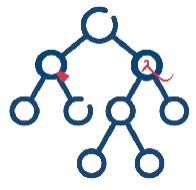
\includegraphics[height=1.0cm]{msca_logo.png}}%
    \end{center}

    \vspace{0.6cm}

    % Main title with Q logos on sides (with clickable links)
    \begin{center}
        \begin{minipage}{0.1\textwidth}
            \centering
            \href{https://quantlet.com}{
\includegraphics[height=1.1cm]{ql_logo.png}}
        \end{minipage}%
        \begin{minipage}{0.78\textwidth}
            \centering
            {\LARGE\bfseries\usebeamercolor[fg]{title}\inserttitle}

            \vspace{0.3cm}

            {\usebeamerfont{subtitle}\usebeamercolor[fg]{title}\insertsubtitle}
        \end{minipage}%
        \begin{minipage}{0.1\textwidth}
            \centering
            \href{https://quantinar.com}{
\includegraphics[height=1.1cm]{qr_logo.png}}
        \end{minipage}
    \end{center}

    \vspace{0.6cm}

    % Authors (left aligned)
    \hspace{0.5cm}{\usebeamerfont{author}\insertauthor}

    \vspace{0.3cm}

    % Institute/Affiliations (left aligned)
    \hspace{0.5cm}\begin{minipage}[t]{0.9\textwidth}
        \raggedright\small\insertinstitute
    \end{minipage}
}

%=============================================================================
% THEOREM ENVIRONMENTS
%=============================================================================
\theoremstyle{definition}
\setbeamertemplate{theorems}[numbered]
\ifdefined\sfmlang
\newtheorem{defn}{Definiție}
\newtheorem{thm}{Teoremă}
\newtheorem{prop}{Propoziție}
\newtheorem{rmk}{Observație}
\else
\newtheorem{defn}{Definition}
\newtheorem{thm}{Theorem}
\newtheorem{prop}{Proposition}
\newtheorem{rmk}{Remark}
\fi

%=============================================================================
% CENTRED MINIPAGE (no extra vertical space)
%=============================================================================
\newenvironment{cminipage}[1]{%
    \par\noindent\hfill\begin{minipage}{#1}\ignorespaces
}{%
    \end{minipage}\hfill\null\par
}

%=============================================================================
% CUSTOM COMMANDS
%=============================================================================
\newcommand{\E}{\mathbb{E}}
\newcommand{\Var}{\text{Var}}
\newcommand{\Cov}{\text{Cov}}
\newcommand{\Corr}{\text{Corr}}
\newcommand{\R}{\mathbb{R}}
\newcommand{\N}{\mathbb{N}}
\newcommand{\Z}{\mathbb{Z}}
\newcommand{\B}{\mathbf{B}}
\newcommand{\imark}{\textcolor{MainBlue}{\textbullet}}
\newcommand{\RMSE}{\text{RMSE}}
\newcommand{\MAE}{\text{MAE}}
\newcommand{\MAPE}{\text{MAPE}}

 se definește
%   \newcommand{\coursename}{Statistics of Financial Markets}      (EN)
%   \newcommand{\coursename}{Statistica piețelor financiare}       (RO)  și  \def\sfmlang{ro}
% Fișierele .tex se află în EN/Courses, EN/Seminars, RO/Cursuri, RO/Seminarii (două niveluri sub rădăcină).
% Deck-urile sînt generate de latex/build_chapterN.py / build_seminarN.py (vezi latex/sfm_build.py).

\documentclass[9pt, aspectratio=169, t]{beamer}
\providecommand{\coursename}{Statistics of Financial Markets}

% Ensure content fits on slides
\setbeamersize{text margin left=8mm, text margin right=8mm}

%=============================================================================
% THEME AND STYLE CONFIGURATION
%=============================================================================
\usetheme{default}
% Using default theme for clean header/footer control

% Color Palette (matching Redispatch PDF)
\definecolor{MainBlue}{RGB}{26, 58, 110}
\definecolor{AccentBlue}{RGB}{26, 58, 110}
\definecolor{IDAred}{RGB}{205, 0, 0}
\definecolor{DarkGray}{RGB}{51, 51, 51}
\definecolor{MediumGray}{RGB}{128, 128, 128}
\definecolor{LightGray}{RGB}{248, 248, 248}
\definecolor{VeryLightGray}{RGB}{235, 235, 235}
\definecolor{KeynoteGray}{RGB}{218, 218, 218}
\definecolor{SectionGray}{RGB}{120, 120, 120}
\definecolor{FooterGray}{RGB}{100, 100, 100}
\definecolor{Crimson}{RGB}{220, 53, 69}
\definecolor{Forest}{RGB}{46, 125, 50}
\definecolor{Amber}{RGB}{181, 133, 63}
\definecolor{Orange}{RGB}{230, 126, 34}
\definecolor{Purple}{RGB}{142, 68, 173}

% Gradient background (exact Keynote 315° gradient: white to RGB 218,218,218)
\setbeamertemplate{background}{%
    \begin{tikzpicture}[remember picture, overlay]
        \shade[shading=axis, shading angle=315,
        top color=white, bottom color=KeynoteGray]
        (current page.south west) rectangle (current page.north east);
    \end{tikzpicture}%
}
% Fallback solid color for compatibility
\setbeamercolor{background canvas}{bg=}

\setbeamercolor{palette primary}{bg=MainBlue, fg=white}
\setbeamercolor{palette secondary}{bg=MainBlue!85, fg=white}
\setbeamercolor{palette tertiary}{bg=MainBlue!70, fg=white}
\setbeamercolor{structure}{fg=MainBlue}
\setbeamercolor{title}{fg=IDAred}
\setbeamercolor{frametitle}{fg=IDAred, bg=}
\setbeamercolor{block title}{bg=MainBlue, fg=white}
\setbeamercolor{block body}{bg=VeryLightGray, fg=DarkGray}
\setbeamercolor{block title alerted}{bg=Crimson, fg=white}
\setbeamercolor{block body alerted}{bg=Crimson!8, fg=DarkGray}
\setbeamercolor{block title example}{bg=Forest, fg=white}
\setbeamercolor{block body example}{bg=Forest!8, fg=DarkGray}
\setbeamercolor{item}{fg=MainBlue}

% Footer colors (override Madrid theme blue)
\setbeamercolor{author in head/foot}{fg=FooterGray, bg=}
\setbeamercolor{title in head/foot}{fg=FooterGray, bg=}
\setbeamercolor{date in head/foot}{fg=FooterGray, bg=}
\setbeamercolor{section in head/foot}{fg=FooterGray, bg=}
\setbeamercolor{subsection in head/foot}{fg=FooterGray, bg=}

% Bullet styles (apply everywhere including blocks)
\setbeamertemplate{itemize item}{\color{MainBlue}$\boxdot$}
\setbeamertemplate{itemize subitem}{\color{MainBlue}$\blacktriangleright$}
\setbeamertemplate{itemize subsubitem}{\color{MainBlue}\tiny$\bullet$}
\setbeamertemplate{itemize/enumerate body begin}{\normalsize}
\setbeamertemplate{itemize/enumerate subbody begin}{\normalsize}

% Item spacing - compact style
\setlength{\leftmargini}{10pt}       % Level 1: minimal indent
\setlength{\leftmarginii}{10pt}      % Level 2: minimal additional indent
% Compact list spacing (zero extra space before/after lists in blocks)
\makeatletter
\def\@listi{\leftmargin\leftmargini \topsep 0pt \parsep 0pt \itemsep 0pt}
\def\@listii{\leftmargin\leftmarginii \topsep 0pt \parsep 0pt \itemsep 0pt}
\makeatother

\setbeamertemplate{navigation symbols}{}

%=============================================================================
% CUSTOM HEADLINE
%=============================================================================
\setbeamertemplate{headline}{%
    \vskip10pt%
    \hbox to \paperwidth{%
        \hskip0.5cm%
        {\small\color{FooterGray}\renewcommand{\hyperlink}[2]{##2}\insertsectionhead}%
        \hfill%
        \textcolor{FooterGray}{\small\insertframenumber}%
        \hskip0.5cm%
    }%
    \vskip4pt%
    {\color{FooterGray}\hrule height 0.4pt}%
}

%=============================================================================
% CUSTOM FOOTER
%=============================================================================
\usepackage{fontawesome5}

\setbeamertemplate{footline}{%
    {\color{FooterGray}\hrule height 0.4pt}%
    \vskip4pt%
    \hbox to \paperwidth{%
        \hskip0.5cm%
        \textcolor{FooterGray}{\small\coursename}%
        \hfill%
        \raisebox{-0.1em}{%
            \begin{tikzpicture}[x=0.08em, y=0.08em, line width=0.4pt]
                \draw[FooterGray] (0,3) -- (1,4) -- (2,3.5) -- (3,5) -- (4,4) -- (5,6) -- (6,5.5) -- (7,4) -- (8,5) -- (9,7) -- (10,6) -- (11,5) -- (12,6.5) -- (13,8) -- (14,7) -- (15,6) -- (16,7.5) -- (17,9) -- (18,8) -- (19,7) -- (20,8.5) -- (21,10) -- (22,9) -- (23,8) -- (24,9.5);
            \end{tikzpicture}%
        }%
        \hskip0.5cm%
    }%
    \vskip6pt%
}

%=============================================================================
% PACKAGES
%=============================================================================
\usepackage[utf8]{inputenc}
\DeclareUnicodeCharacter{03B1}{\ensuremath{\alpha}}
\usepackage[T1]{fontenc}
\usepackage{amsmath, amssymb, amsthm}
\usepackage{mathtools}
\usepackage{bm}
\usepackage{tikz}
\usetikzlibrary{arrows.meta, positioning, shapes, calc, decorations.pathreplacing, shadings}
\usepackage{booktabs}
\usepackage{multirow}
\usepackage{array}
\usepackage{graphicx}
\usepackage{hyperref}
\usepackage{colortbl}
\usepackage{listings}
\lstset{language=Python, basicstyle=\ttfamily\scriptsize, keywordstyle=\color{MainBlue}\bfseries,
  commentstyle=\color{Forest}, stringstyle=\color{Crimson}, breaklines=true,
  frame=none, backgroundcolor=\color{VeryLightGray}, xleftmargin=2mm}
\hypersetup{colorlinks=true, linkcolor=MainBlue, urlcolor=MainBlue}
\graphicspath{{../../logos/}{../../charts/}{../../photos/}}
\usepackage{xcolor}
\hfuzz=2pt  % Suppress tiny overfull warnings (<2pt)
\vfuzz=2pt  % Suppress tiny vertical overfull warnings (<2pt)

%=============================================================================
% QUANTLET COMMANDS
%   \quantlet{<displayed name>}{<url>}       (generic, compatible with the older SFM decks)
%   \sfmquantlet{Ch_05}{SFM_ch5_garch}       -> https://github.com/danpele/SFM/tree/main/Quantlets/Ch_05/SFM_ch5_garch
%   \qlurl{<folder>} is defined per chapter by the generator (Quantlets/Ch_NN/<folder>)
%=============================================================================
\newcommand{\sfmrepo}{https://github.com/danpele/SFM}
\newcommand{\sfmqlbase}{https://github.com/danpele/SFM/tree/main/Quantlets}
\newcommand{\quantlet}[2]{%
    \hfill\href{#2}{%
        \raisebox{-0.15em}{
\includegraphics[height=0.7em]{ql_logo.png}}%
        \textcolor{MainBlue}{\tiny\ #1}%
    }%
}
\newcommand{\sfmquantlet}[2]{\quantlet{\detokenize{#2}}{\sfmqlbase/#1/#2}}

%=============================================================================
% NOTEBOOKS (Google Colab)
%   \colaburl{notebooks/EN/chapter5_seminar_notebook.ipynb} -> the Colab link of a file in the SFM repo
%   \nb: the chapter notebook (each seminar deck redefines it with \renewcommand)
%=============================================================================
\newcommand{\colaburl}[1]{https://colab.research.google.com/github/danpele/SFM/blob/main/#1}
\newcommand{\nb}{https://colab.research.google.com/github/danpele/SFM/tree/main/notebooks/EN}
\newcommand{\nbname}{notebooks/EN}

%=============================================================================
% SLIDE HELPERS (used by the generators; the same as in MFM)
%=============================================================================
% local font size for list bodies (the preamble forces \normalsize)
\newcommand{\itemsize}[1]{\setbeamertemplate{itemize/enumerate body begin}{#1}\setbeamertemplate{itemize/enumerate subbody begin}{#1}}
\newcommand{\intitle}[1]{{\hypersetup{urlcolor=white}#1}}   % white links inside coloured title bars
\newcommand{\imgcap}[1]{{\scriptsize #1}\\[0.5mm]}          % caption under a photo
\newcommand{\imgcredit}[2]{{\tiny\color{FooterGray}\href{#1}{#2}}}   % image credit: source URL, author/licence
\newcommand{\aiprompt}[1]{{\ttfamily\color{MainBlue}#1}}     % a prompt to an AI assistant

%=============================================================================
% SEMINARS: student version by default; the instructor wrapper *_solutions.tex sets \solutionstrue
%=============================================================================
\makeatletter\@ifundefined{ifsolutions}{\expandafter\newif\csname ifsolutions\endcsname}{}\makeatother
\newcommand{\solonly}[1]{\ifsolutions #1\fi}
\newcommand{\propsub}{\ifsolutions\else\framesubtitle{\ifdefined\sfmlang Rezolvarea se discută la seminar\else Solution discussed in class\fi}\fi}

%=============================================================================
% APPENDIX AND CHAPTER LINKS (latex/appendix_links.py writes the calls; it also re-declares these
% macros before \begin{document}, so the decks compile with or without this preamble block)
%=============================================================================
\providecommand{\sfmapplink}[3]{\hypertarget{#2}{}\hyperlink{#1}{\beamergotobutton{#3}}}
\providecommand{\sfmappback}[2]{\begin{tikzpicture}[remember picture,overlay]\node[anchor=south east] at ([xshift=-3mm,yshift=7mm]current page.south east){\hyperlink{#1}{\beamerreturnbutton{#2}}};\end{tikzpicture}}
\providecommand{\sfmchlink}[2]{\href{#1}{#2}}
\providecommand{\sfmchlinkt}[2]{\href{#1}{\usebeamercolor[fg]{frametitle}#2}}

%=============================================================================
% QUANTINAR COMMAND: link către un curs Quantinar (subiecte avansate)
%=============================================================================
\newcommand{\quantinar}[2]{%
    \href{#2}{%
        \raisebox{-0.15em}{
\includegraphics[height=0.8em]{qr_logo.png}}%
        \textcolor{MainBlue}{\scriptsize\ #1}%
    }%
}

%=============================================================================
% CUSTOM TITLE PAGE
%=============================================================================
\defbeamertemplate*{title page}{hybrid}[1][]
{
    \vspace{0.2cm}
    % Logos row - top header (with clickable links)
    \begin{center}
        \href{https://www.ase.ro}{
\includegraphics[height=1.0cm]{ase_logo.png}}\hspace{0.3cm}%
        \href{https://theida.net}{
\includegraphics[height=1.0cm]{ida_logo.png}}\hspace{0.3cm}%
        \href{https://blockchain-research-center.com}{
\includegraphics[height=1.0cm]{brc_logo.png}}\hspace{0.3cm}%
        \href{https://www.ai4efin.ase.ro}{
\includegraphics[height=1.0cm]{ai4efin_logo.png}}\hspace{0.3cm}%
        \href{https://ipe.ro/new}{
\includegraphics[height=1.0cm]{acad_logo.png}}\hspace{0.3cm}%
        \href{https://www.digital-finance-msca.com}{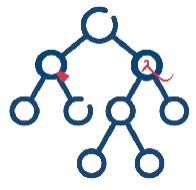
\includegraphics[height=1.0cm]{msca_logo.png}}%
    \end{center}

    \vspace{0.6cm}

    % Main title with Q logos on sides (with clickable links)
    \begin{center}
        \begin{minipage}{0.1\textwidth}
            \centering
            \href{https://quantlet.com}{
\includegraphics[height=1.1cm]{ql_logo.png}}
        \end{minipage}%
        \begin{minipage}{0.78\textwidth}
            \centering
            {\LARGE\bfseries\usebeamercolor[fg]{title}\inserttitle}

            \vspace{0.3cm}

            {\usebeamerfont{subtitle}\usebeamercolor[fg]{title}\insertsubtitle}
        \end{minipage}%
        \begin{minipage}{0.1\textwidth}
            \centering
            \href{https://quantinar.com}{
\includegraphics[height=1.1cm]{qr_logo.png}}
        \end{minipage}
    \end{center}

    \vspace{0.6cm}

    % Authors (left aligned)
    \hspace{0.5cm}{\usebeamerfont{author}\insertauthor}

    \vspace{0.3cm}

    % Institute/Affiliations (left aligned)
    \hspace{0.5cm}\begin{minipage}[t]{0.9\textwidth}
        \raggedright\small\insertinstitute
    \end{minipage}
}

%=============================================================================
% THEOREM ENVIRONMENTS
%=============================================================================
\theoremstyle{definition}
\setbeamertemplate{theorems}[numbered]
\ifdefined\sfmlang
\newtheorem{defn}{Definiție}
\newtheorem{thm}{Teoremă}
\newtheorem{prop}{Propoziție}
\newtheorem{rmk}{Observație}
\else
\newtheorem{defn}{Definition}
\newtheorem{thm}{Theorem}
\newtheorem{prop}{Proposition}
\newtheorem{rmk}{Remark}
\fi

%=============================================================================
% CENTRED MINIPAGE (no extra vertical space)
%=============================================================================
\newenvironment{cminipage}[1]{%
    \par\noindent\hfill\begin{minipage}{#1}\ignorespaces
}{%
    \end{minipage}\hfill\null\par
}

%=============================================================================
% CUSTOM COMMANDS
%=============================================================================
\newcommand{\E}{\mathbb{E}}
\newcommand{\Var}{\text{Var}}
\newcommand{\Cov}{\text{Cov}}
\newcommand{\Corr}{\text{Corr}}
\newcommand{\R}{\mathbb{R}}
\newcommand{\N}{\mathbb{N}}
\newcommand{\Z}{\mathbb{Z}}
\newcommand{\B}{\mathbf{B}}
\newcommand{\imark}{\textcolor{MainBlue}{\textbullet}}
\newcommand{\RMSE}{\text{RMSE}}
\newcommand{\MAE}{\text{MAE}}
\newcommand{\MAPE}{\text{MAPE}}



\newcommand{\qlurl}[1]{https://github.com/danpele/SFM/tree/main/Quantlets/Ch_04/#1}
\renewcommand{\nb}{\colaburl{notebooks/EN/chapter4_seminar_notebook.ipynb}}
\renewcommand{\nbname}{chapter4\_seminar\_notebook.ipynb}
% left column: full width in the student version, narrower next to the solution
\newcommand{\taskw}{\ifsolutions 0.47\textwidth\else 0.96\textwidth\fi}
\newcommand{\solw}{\ifsolutions 0.49\textwidth\else 0pt\fi}

% Clickable citations (DOIs verified via Crossref)

\newcommand{\refFHH}{\href{https://doi.org/10.1007/978-3-030-13751-9}{Franke, Härdle \& Hafner (2019)}}
\newcommand{\refFHHex}{\href{https://doi.org/10.1007/978-3-642-33929-5}{Borak, Härdle \& López-Cabrera (2013)}}
\newcommand{\refKolmogorov}{\href{https://doi.org/10.1007/978-3-642-49888-6}{Kolmogoroff (1933)}}
\newcommand{\refBachelier}{\href{https://doi.org/10.24033/asens.476}{Bachelier (1900)}}
\newcommand{\refEinstein}{\href{https://doi.org/10.1002/andp.19053220806}{Einstein (1905)}}
\newcommand{\refWiener}{\href{https://doi.org/10.1002/sapm192321131}{Wiener (1923)}}
\newcommand{\refOsborne}{\href{https://doi.org/10.1287/opre.7.2.145}{Osborne (1959)}}
\newcommand{\refBS}{\href{https://doi.org/10.1086/260062}{Black \& Scholes (1973)}}
\newcommand{\refCRR}{\href{https://doi.org/10.1016/0304-405X(79)90015-1}{Cox, Ross \& Rubinstein (1979)}}
\newcommand{\refMU}{\href{https://doi.org/10.1080/01621459.1949.10483310}{Metropolis \& Ulam (1949)}}
\newcommand{\refMarsaglia}{\href{https://doi.org/10.1073/pnas.61.1.25}{Marsaglia (1968)}}
\newcommand{\refMT}{\href{https://doi.org/10.1145/272991.272995}{Matsumoto \& Nishimura (1998)}}
\newcommand{\refGlasserman}{\href{https://doi.org/10.1007/978-0-387-21617-1}{Glasserman (2003)}}
\newcommand{\refEngle}{\href{https://doi.org/10.2307/1912773}{Engle (1982)}}
\newcommand{\refBollerslev}{\href{https://doi.org/10.1016/0304-4076(86)90063-1}{Bollerslev (1986)}}
\newcommand{\refFama}{\href{https://doi.org/10.2307/2325486}{Fama (1970)}}
\newcommand{\refCont}{\href{https://doi.org/10.1080/713665670}{Cont (2001)}}
\newcommand{\refPeleCrypto}{\href{https://doi.org/10.1080/1351847X.2021.1960403}{Pele et al.\ (2023)}}
\newcommand{\refWang}{\href{https://doi.org/10.1038/s41586-023-06221-2}{Wang et al.\ (2023)}}

\title[Statistics of Financial Markets]{Statistics of Financial Markets}
\subtitle{Seminar 4: Probability\ifsolutions\ (instructor version)\fi}
\author[D.T. Pele]{Daniel Traian PELE}
\institute{Bucharest University of Economic Studies\\
IDA Institute Digital Assets\\
Blockchain Research Center\\
AI4EFin Artificial Intelligence for Energy Finance\\
Romanian Academy, Institute for Economic Forecasting\\
MSCA Digital Finance}
\date{}

%=============================================================================
\providecommand{\sfmapplink}[3]{\hypertarget{#2}{}\hyperlink{#1}{\beamergotobutton{#3}}}  % APPLINKS-MACROS
\providecommand{\sfmappback}[2]{\begin{tikzpicture}[remember picture,overlay]\node[anchor=south east] at ([xshift=-3mm,yshift=7mm]current page.south east){\hyperlink{#1}{\beamerreturnbutton{#2}}};\end{tikzpicture}}  % APPLINKS-MACROS
\providecommand{\sfmchlink}[2]{\href{#1}{#2}}  % APPLINKS-MACROS
\providecommand{\sfmchlinkt}[2]{\href{#1}{\usebeamercolor[fg]{frametitle}#2}}  % APPLINKS-MACROS
\begin{document}
%=============================================================================

{
\setbeamertemplate{headline}{}
\setbeamertemplate{footline}{}
\begin{frame}[noframenumbering]
    \titlepage
\end{frame}
}
% BEGIN-ACRONYMS (generat de latex/acronyms.py; nu editati manual)
\begin{frame}{Acronyms used in this material}
\setbeamertemplate{itemize/enumerate body begin}{\tiny}
\begin{columns}[T]
\begin{column}{0.49\textwidth}
\begin{itemize}\setlength{\itemsep}{0pt}
    \item \textbf{AI}: Artificial Intelligence
    \item \textbf{AR}: AutoRegressive (model)
    \item \textbf{BET}: Bucharest Exchange Trading (index)
    \item \textbf{CDF}: Cumulative Distribution Function
    \item \textbf{EODHD}: EOD Historical Data (market-data provider)
    \item \textbf{GARCH}: Generalised AutoRegressive Conditional Heteroskedasticity
    \item \textbf{GBM}: Gradient Boosting Machine
    \item \textbf{LCG}: Linear Congruential Generator
    \item \textbf{PCG64}: Permuted Congruential Generator, 64-bit (NumPy default)
    \item \textbf{PMF}: Probability Mass Function
    \item \textbf{RANDU}: RANDU (IBM random number generator of the 1960s)
\end{itemize}
\end{column}
\begin{column}{0.49\textwidth}
\end{column}
\end{columns}
\end{frame}
% END-ACRONYMS

\begin{frame}{Today's Question and Route}
\itemsize{\small}
\begin{itemize}
    \item \textbf{Question}: how do we describe, condition and simulate random returns and prices?
    \begin{itemize}
        \item this seminar comes \textbf{before} Lecture 4: the section ``What You Need for Today'' gives every definition the tasks use
    \end{itemize}
    \item Route
    \begin{itemize}
        \item Part A: moments, joint tables, conditioning, binomial trees, AR(1), inverse transform and GBM on paper
        \item Part B: dependence in real returns, Monte Carlo, random number generators and GBM against data, each with an interpretation question
        \item Part C: an open question for a project and an AI answer to audit
    \end{itemize}
    \item Notebook for today: \href{\nb}{open the seminar notebook in Google Colab}; each task names its notebook section
    \item Nothing is handed in: the seminar is for practice; the solutions of [Proposed] tasks are discussed in class
\end{itemize}
\end{frame}

\begin{frame}{Exercise Map}
\itemsize{\small}
\begin{center}
\footnotesize
\begin{tabular}{>{\raggedright\arraybackslash}p{1.0cm}>{\raggedright\arraybackslash}p{7.6cm}>{\raggedright\arraybackslash}p{1.9cm}>{\raggedright\arraybackslash}p{1.4cm}}
\toprule
\textbf{Task} & \textbf{Question} & \textbf{Type} & \textbf{Model} \\
\midrule
A1, A2 & moments of a discrete return; is an uncorrelated pair independent? & Solved, Proposed & A1 \\
A3, A4 & portfolio volatility; a two-regime model and the law of total variance & Solved, Proposed & A3 \\
A5, A6 & a binomial tree; random walk, martingale and AR(1) & Solved, Proposed & A5 \\
A7, A8 & inverse transform by hand; GBM and the Wiener process & Solved, Proposed & A7 \\
B1, B2 & are returns independent? conditional mean and variance & Solved, Proposed & B1 \\
B3, B4 & a loss probability by Monte Carlo; testing a random number generator & Solved, Proposed & B3 \\
B5, B6 & GBM against the BET; does variance grow linearly with the horizon? & Solved, Proposed & B5 \\
C1, C2 & how often is there a bad year? what is wrong in an AI answer? & Proposed & B3, B5 \\
\bottomrule
\end{tabular}
\end{center}
\begin{itemize}
    \item \textbf{[Solved]}: full solution in the slides and in the notebook, a model to follow; \textbf{[Proposed]}: you solve it, following the model
\end{itemize}
\end{frame}

\begin{frame}{Data Used}
\itemsize{\small}
\begin{center}
\footnotesize
\begin{tabular}{llll}
\toprule
\textbf{Series} & \textbf{Source} & \textbf{Price used} & \textbf{Period} \\
\midrule
S\&P 500, DAX, BET & EODHD & close & 2000--2026 \\
Bitcoin & EODHD & close, 7 days a week & 2014--2026 \\
\bottomrule
\end{tabular}
\end{center}
\begin{itemize}
    \item Daily log returns in \%: $r_t = 100\,(\ln P_t - \ln P_{t-1})$
    \item Weekends and repeated holiday closes are dropped (except Bitcoin); each series on its own calendar
    \item Simulations use NumPy's default generator with fixed seeds, so every number can be reproduced
\end{itemize}
\end{frame}


%=============================================================================
\section{What You Need for Today}
%=============================================================================

\begin{frame}{What You Need for Today (1/4): Random Variables and Moments}
\itemsize{\footnotesize}
\begin{itemize}
    \item Discrete $X$: \textbf{PMF} (probability mass function) $p(x_i) = P(X = x_i)$; continuous $X$: \textbf{PDF} (probability density function) $f$
    \begin{itemize}
        \item \textbf{CDF} (cumulative distribution function): $F(x) = P(X \le x)$; quantile $q_\alpha = F^{-1}(\alpha)$
    \end{itemize}
    \item $E[X] = \sum x_i p(x_i)$ or $\int x f(x)\,dx$; $\text{Var}(X) = E[X^2] - (E[X])^2$
    \item $\text{Cov}(X, Y) = E[XY] - E[X]E[Y]$; $\rho = \text{Cov}/(\sigma_X\sigma_Y)$; $\text{Var}(aX + bY) = a^2\sigma_X^2 + b^2\sigma_Y^2 + 2ab\,\text{Cov}$
    \item \textbf{Independent}: $P(X = x, Y = y) = P(X = x)P(Y = y)$ for every cell; independent $\Rightarrow$ uncorrelated, not conversely
    \begin{itemize}
        \item the i.i.d. band for a sample correlation: $\pm 1.96/\sqrt{n}$
    \end{itemize}
\end{itemize}
\end{frame}

\begin{frame}{What You Need for Today (2/4): Conditioning}
\itemsize{\footnotesize}
\begin{itemize}
    \item $P(A \mid B) = P(A \cap B)/P(B)$; $E[Y \mid X]$: the mean of $Y$ once $X$ is known, the best forecast of $Y$ from $X$
    \item \textbf{Tower property}: $E[E[Y \mid X]] = E[Y]$
    \item \textbf{Law of total variance}: $\text{Var}(Y) = E[\text{Var}(Y \mid X)] + \text{Var}(E[Y \mid X])$
    \item For returns: $\mu_t = E[r_t \mid \mathcal{F}_{t-1}]$ and $\sigma_t^2 = \text{Var}(r_t \mid \mathcal{F}_{t-1})$, with $\mathcal{F}_{t-1}$ the information up to yesterday
    \begin{itemize}
        \item a changing $\sigma_t$ is what GARCH models (Chapter 9)
    \end{itemize}
    \item A mixture of Normals with different variances has kurtosis above 3: $E[X^4] = 3\sigma^4$ for $N(0, \sigma^2)$
\end{itemize}
\end{frame}

\begin{frame}{What You Need for Today (3/4): Processes}
\itemsize{\footnotesize}
\begin{itemize}
    \item \textbf{White noise}: mean 0, variance $\sigma^2$, uncorrelated over time; \textbf{i.i.d.} noise: independent and identically distributed
    \item \textbf{Random walk}: $S_t = S_{t-1} + \varepsilon_t$, $E[S_t] = S_0$, $\text{Var}(S_t) = t\sigma^2$
    \item \textbf{Martingale}: $E[X_{t+1} \mid \mathcal{F}_t] = X_t$ (a fair game)
    \item \textbf{AR(1)}: $X_t = c + \phi X_{t-1} + \varepsilon_t$, $|\phi| < 1$: mean $c/(1 - \phi)$, variance $\sigma^2/(1 - \phi^2)$, $\rho(h) = \phi^h$
    \item \textbf{Binomial tree}: up by $u$ with probability $p$, down by $d$; after $n$ steps $S_n = S_0u^Kd^{n-K}$, $K \sim B(n, p)$
    \begin{itemize}
        \item $E[S_n] = S_0(pu + (1 - p)d)^n$; fair game for $p^* = (1 - d)/(u - d)$
    \end{itemize}
\end{itemize}
\end{frame}

\begin{frame}{What You Need for Today (4/4): Simulation, Wiener and GBM}
\itemsize{\footnotesize}
\begin{itemize}
    \item \textbf{Inverse transform}: $U \sim U(0, 1)$ $\Rightarrow$ $F^{-1}(U)$ has CDF $F$; exponential: $-\ln(1 - U)/\lambda$; Normal: $\mu + \sigma\Phi^{-1}(U)$
    \item \textbf{LCG} (linear congruential generator): $x_{k+1} = (ax_k + c) \bmod M$, $u_k = x_k/M$
    \item \textbf{Monte Carlo}: $\hat p = $ share of simulations in the event; standard error $\sqrt{p(1 - p)/N}$
    \item \textbf{Wiener process}: $W(0) = 0$, independent increments, $W(t) - W(s) \sim N(0, t - s)$; $\text{Cov}(W(s), W(t)) = \min(s, t)$
    \item \textbf{GBM} (geometric Brownian motion): $S_T = S_0\exp((\mu - \sigma^2/2)T + \sigma W_T)$
    \begin{itemize}
        \item mean $S_0e^{\mu T}$, median $S_0e^{(\mu - \sigma^2/2)T}$; daily log returns i.i.d. Normal
        \item maximum drawdown: $\min_t(P_t/\max_{s \le t}P_s - 1)$, the largest fall from a running peak
    \end{itemize}
\end{itemize}
\end{frame}


%=============================================================================
\section{Part A: Computations and Derivations on Paper}
%=============================================================================

\begin{frame}{A1: Moments of a Discrete Return [Solved]}
\itemsize{\footnotesize}
\begin{columns}[T]
\begin{column}{0.47\textwidth}
\begin{block}{Task}
\begin{itemize}
    \item A stock's daily return $X$ (in \%) takes the values $-3$, $0$ and $2$ with probabilities $0.2$, $0.3$ and $0.5$.
    \item 1. Compute $E[X]$, $E[X^2]$, $\text{Var}(X)$ and the standard deviation.
    \item 2. Write the CDF $F(x)$ for every $x$.
    \item 3. Compute $P(X < 0)$ and the median.
    \item Report: four moments, the CDF and two numbers.
\end{itemize}
\end{block}
\end{column}
\begin{column}{0.49\textwidth}
\begin{exampleblock}{Solution}
\begin{itemize}
    \item 1. $E[X] = -0.6 + 0 + 1 = 0.40$; $E[X^2] = 1.8 + 2 = 3.80$; $\text{Var} = 3.80 - 0.40^2 = 3.64$; s.d. $1.908$
    \item 2. $F(x) = 0$ for $x < -3$; $0.2$ on $[-3, 0)$; $0.5$ on $[0, 2)$; $1$ for $x \ge 2$
    \item 3. $P(X < 0) = 0.2$; median $= \inf\{x : F(x) \ge 0.5\} = 0$
    \item The mean is positive although a loss is possible: risk and expected return are different questions.
\end{itemize}
\end{exampleblock}
\end{column}
\end{columns}
\end{frame}

\begin{frame}{A2: Uncorrelated but Dependent [Proposed]}
\propsub
\itemsize{\scriptsize}
\begin{columns}[T]
\begin{column}{\taskw}
\begin{block}{Task}
\begin{itemize}
    \item $X$ = market move ($-1$ fall, $0$ flat, $+1$ rise); $Y = 1$ if the day is ``large''. Joint probabilities: $P(-1, 1) = 0.25$, $P(0, 0) = 0.5$, $P(1, 1) = 0.25$, all other cells 0. Model: A1.
    \item 1. Compute the marginal distributions of $X$ and $Y$ and their means.
    \item 2. Compute $\text{Cov}(X, Y)$ and $\rho$.
    \item 3. Decide whether $X$ and $Y$ are independent, using one cell of the table.
    \item 4. Compute $\text{Var}(X + Y)$.
    \item Report: two marginals, $\rho$, a verdict and a variance.
\end{itemize}
\end{block}
\end{column}
\begin{column}{\solw}
\solonly{%
\begin{exampleblock}{Solution}
\begin{itemize}
    \item 1. $X$: $0.25, 0.5, 0.25$, $E[X] = 0.00$; $Y$: $0.5, 0.5$, $E[Y] = 0.50$
    \item 2. $E[XY] = -0.25 + 0.25 = 0.00$, $\text{Cov} = 0.00$, $\rho = 0$
    \item 3. $P(X = 0, Y = 0) = 0.5 \ne P(X = 0)P(Y = 0) = 0.25$: dependent ($Y = |X|$)
    \item 4. $\text{Var}(X) + \text{Var}(Y) + 2\,\text{Cov} = 0.50 + 0.25 + 0 = 0.75$
    \item The same structure as returns and their absolute values.
\end{itemize}
\end{exampleblock}
}
\end{column}
\end{columns}
\end{frame}

\begin{frame}{A3: Volatility of a Two-Asset Portfolio [Solved]}
\itemsize{\footnotesize}
\begin{columns}[T]
\begin{column}{0.47\textwidth}
\begin{block}{Task}
\begin{itemize}
    \item Two assets with annual volatilities $\sigma_1 = 20\%$ and $\sigma_2 = 30\%$; weights $0.6$ and $0.4$.
    \item 1. Compute the portfolio volatility for $\rho = 0.3$.
    \item 2. Repeat for $\rho = 0$, $\rho = -0.5$ and $\rho = 1$.
    \item 3. Explain when the portfolio is less risky than the weighted average of the two volatilities.
    \item Report: four volatilities and one sentence.
\end{itemize}
\end{block}
\end{column}
\begin{column}{0.49\textwidth}
\begin{exampleblock}{Solution}
\begin{itemize}
    \item 1. $\sigma_p^2 = 0.36 \times 400 + 0.16 \times 900 + 2 \times 0.24 \times 0.3 \times 600 = 374.4$; $\sigma_p = 19.35\%$
    \item 2. $\rho = 0$: $16.97\%$; $\rho = -0.5$: $12.00\%$; $\rho = 1$: $24.00\%$
    \item 3. Only $\rho = 1$ gives the weighted average $0.6 \times 20 + 0.4 \times 30 = 24\%$; every $\rho < 1$ diversifies.
\end{itemize}
\end{exampleblock}
\end{column}
\end{columns}
\end{frame}

\begin{frame}{A4: Two Regimes and the Law of Total Variance [Proposed]}
\propsub
\itemsize{\scriptsize}
\begin{columns}[T]
\begin{column}{\taskw}
\begin{block}{Task}
\begin{itemize}
    \item A day is calm with probability $0.8$, $r \mid \text{calm} \sim N(0, 0.8^2)$, and turbulent otherwise, $r \mid \text{turbulent} \sim N(0, 2^2)$ (in \%). Model: A3.
    \item 1. Use the law of total variance to compute $\text{Var}(r)$ and the standard deviation.
    \item 2. Compute $E[r^4]$ with $E[Z^4] = 3\sigma^4$ in each regime, then the kurtosis $E[r^4]/\text{Var}(r)^2$.
    \item 3. Explain why the mixture has heavy tails although each regime is Normal.
    \item Report: a variance, a kurtosis and one sentence.
\end{itemize}
\end{block}
\end{column}
\begin{column}{\solw}
\solonly{%
\begin{exampleblock}{Solution}
\begin{itemize}
    \item 1. $E[\text{Var}] = 0.8 \times 0.64 + 0.2 \times 4 = 1.312$, $\text{Var}(E) = 0$; s.d. $1.145\%$
    \item 2. $E[r^4] = 3(0.8 \times 0.8^4 + 0.2 \times 2^4) = 10.583$; kurtosis $6.15$, excess $3.15$
    \item 3. Large moves come almost only from the turbulent regime; $P(|r| > 4\sigma) = 0.439\%$ vs $0.006\%$ for one Normal
    \item This is the GARCH mechanism in its simplest form.
\end{itemize}
\end{exampleblock}
}
\end{column}
\end{columns}
\end{frame}

\begin{frame}{A5: A Three-Step Binomial Tree [Solved]}
\itemsize{\footnotesize}
\begin{columns}[T]
\begin{column}{0.47\textwidth}
\begin{block}{Task}
\begin{itemize}
    \item $S_0 = 100$, $u = 1.1$, $d = 0.9$, $p = 0.55$, three independent steps.
    \item 1. List the possible values of $S_3$ and their probabilities.
    \item 2. Compute $E[S_3]$ in two ways: from the table and from $S_0(pu + (1 - p)d)^3$.
    \item 3. Compute $P(S_3 < 100)$.
    \item 4. Find the $p^*$ that makes $S_t$ a martingale.
    \item Report: a table, two expectations, a probability, $p^*$.
\end{itemize}
\end{block}
\end{column}
\begin{column}{0.49\textwidth}
\begin{exampleblock}{Solution}
\begin{itemize}
    \item 1. $K = 0..3$ up moves: $72.9, 89.1, 108.9, 133.1$ with $0.0911, 0.3341, 0.4084, 0.1664$ ($\binom{3}{k}p^k(1-p)^{3-k}$)
    \item 2. $E[S_3] = 100 \times 1.01^3 = 103.03$ both ways
    \item 3. $P(K \le 1) = 0.4253$
    \item 4. $p^* = (1 - 0.9)/(1.1 - 0.9) = 0.50$: with $p = 0.55 > p^*$ the price drifts up
\end{itemize}
\end{exampleblock}
\end{column}
\end{columns}
\end{frame}

\begin{frame}{A6: Random Walk, Martingale and AR(1) [Proposed]}
\propsub
\itemsize{\scriptsize}
\begin{columns}[T]
\begin{column}{\taskw}
\begin{block}{Task}
\begin{itemize}
    \item $S_t = S_{t-1} + \varepsilon_t$, $\varepsilon_t$ i.i.d. with mean 0 and variance $\sigma^2$; $X_t = 0.2 + 0.6X_{t-1} + \varepsilon_t$ with $\sigma = 1$. Model: A5.
    \item 1. Compute $E[S_t]$ and $\text{Var}(S_t)$, and show that $S_t$ is a martingale.
    \item 2. Show that $S_t^2 - t\sigma^2$ is also a martingale.
    \item 3. Compute the mean, the variance and $\rho(1), \rho(2), \rho(5)$ of the stationary $X_t$.
    \item 4. Compute $E[X_{t+1} \mid X_t = 2]$ and $\text{Var}(X_{t+1} \mid X_t = 2)$.
    \item Report: two derivations, five moments, a forecast.
\end{itemize}
\end{block}
\end{column}
\begin{column}{\solw}
\solonly{%
\begin{exampleblock}{Solution}
\begin{itemize}
    \item 1. $E[S_t] = S_0$, $\text{Var}(S_t) = t\sigma^2$; $E[S_{t+1} \mid \mathcal{F}_t] = S_t + E[\varepsilon_{t+1}] = S_t$
    \item 2. $E[(S_t + \varepsilon_{t+1})^2 \mid \mathcal{F}_t] = S_t^2 + \sigma^2$, so $E[S_{t+1}^2 - (t+1)\sigma^2 \mid \mathcal{F}_t] = S_t^2 - t\sigma^2$
    \item 3. Mean $0.2/0.4 = 0.50$; variance $1/0.64 = 1.5625$; $\rho = 0.60, 0.36, 0.0778$
    \item 4. $0.2 + 0.6 \times 2 = 1.40$, conditional variance 1: the forecast is pulled back towards the mean 0.50
\end{itemize}
\end{exampleblock}
}
\end{column}
\end{columns}
\end{frame}

\begin{frame}{A7: The Inverse Transform Step by Step [Solved]}
\itemsize{\footnotesize}
\begin{columns}[T]
\begin{column}{0.47\textwidth}
\begin{block}{Task}
\begin{itemize}
    \item You have the uniform numbers $u = 0.3$ and $u = 0.9$ (and $u = 0.15, 0.45, 0.8$ for question 2).
    \item 1. Turn $u = 0.3$ and $u = 0.9$ into exponential draws with rate $\lambda = 0.5$.
    \item 2. Turn $u = 0.15, 0.45, 0.8$ into draws of the return $X$ of A1.
    \item 3. Turn $u = 0.01$ into a draw of $N(0.05, 1.2^2)$.
    \item Report: six simulated values.
\end{itemize}
\end{block}
\end{column}
\begin{column}{0.49\textwidth}
\begin{exampleblock}{Solution}
\begin{itemize}
    \item 1. $x = -\ln(1 - u)/0.5$: $0.713$ and $4.605$
    \item 2. $F^{-1}(u) = \inf\{x : F(x) \ge u\}$ with $F = 0.2, 0.5, 1$: $-3$, $0$ and $2$
    \item 3. $0.05 + 1.2 \times (-2.326) = -2.742$: the 1\% quantile
    \item A large $u$ gives a large draw: the inverse transform keeps the order of the uniforms.
\end{itemize}
\end{exampleblock}
\end{column}
\end{columns}
\end{frame}

\begin{frame}{A8: GBM and the Wiener Process [Proposed]}
\propsub
\itemsize{\scriptsize}
\begin{columns}[T]
\begin{column}{\taskw}
\begin{block}{Task}
\begin{itemize}
    \item An index follows GBM with $\mu = 8\%$, $\sigma = 20\%$ a year, $S_0 = 100$; $W$ is a Wiener process. Model: A7.
    \item 1. Compute the mean and the median of $S_1$ and of $S_5$.
    \item 2. Compute $P(S_T < 100)$ for $T = 1$ and $T = 5$.
    \item 3. Compute the 5\% quantile of $S_1$ and of $S_5$.
    \item 4. Compute $\text{Var}(W(2) - W(0.5))$ and $\text{Cov}(W(1), W(3))$.
    \item Report: eight GBM numbers and two Wiener moments.
\end{itemize}
\end{block}
\end{column}
\begin{column}{\solw}
\solonly{%
\begin{exampleblock}{Solution}
\begin{itemize}
    \item 1. $T = 1$: mean $100e^{0.08} = 108.33$, median $100e^{0.06} = 106.18$; $T = 5$: 149.18 and 134.99
    \item 2. $\Phi(-0.06/0.2) = \Phi(-0.300) = 38.21\%$; $\Phi(-0.3/0.447) = 25.12\%$
    \item 3. $100e^{0.06 - 1.645 \times 0.2} = 76.42$; $100e^{0.3 - 1.645 \times 0.447} = 64.69$
    \item 4. $2 - 0.5 = 1.5$; $\min(1, 3) = 1$
\end{itemize}
\end{exampleblock}
}
\end{column}
\end{columns}
\end{frame}


%=============================================================================
\section{Part B: Simulation, Real Data and Interpretation}
%=============================================================================

\begin{frame}{B1: Are S\&P 500 Returns Independent? [Solved]}
\itemsize{\footnotesize}
\begin{itemize}
\item \textbf{Question}: are the daily returns of the S\&P 500 independent, and what does yesterday tell us about today?
\item \textbf{Inputs}: S\&P 500 closes, 2000--2026, daily log returns in \%
\item \textbf{Tasks}
\begin{enumerate}
    \item Compute $\text{Corr}(r_t, r_{t-1})$ and $\text{Corr}(r_t^2, r_{t-1}^2)$ and compare them with the band $\pm 1.96/\sqrt{n}$.
    \item Split the days into quintiles of $|r_{t-1}|$ and compute the mean and the standard deviation of $r_t$ in each quintile.
    \item Check the law of total variance with the quintiles as groups.
    \item Interpretation: which is predictable from yesterday, the mean or the variance of today's return?
\end{enumerate}
\item \textbf{Report}: two correlations, a table of five quintiles, one decomposition, one sentence
\item Notebook: section B1
\end{itemize}
\end{frame}

\begin{frame}{B1: Solution [Solved]}
\itemsize{\scriptsize}
\begin{columns}[T]
\begin{column}{0.48\textwidth}
\begin{center}
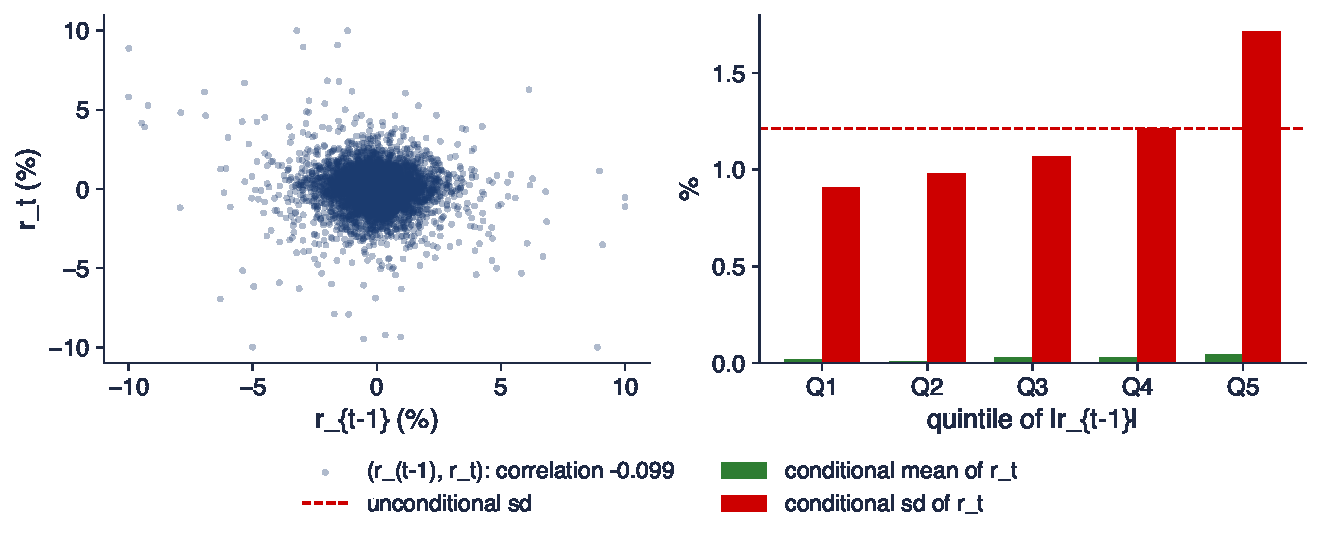
\includegraphics[width=1.0\textwidth,height=0.52\textheight,keepaspectratio]{ch4_sem_b1.pdf}
\end{center}
\vspace{-2mm}

\end{column}
\begin{column}{0.50\textwidth}
\begin{itemize}
    \item $n = 6\,714$, band $\pm 0.024$; $\text{Corr}(r_t, r_{t-1}) = -0.099$; $\text{Corr}(r_t^2, r_{t-1}^2) = 0.313$
    \item Conditional means Q1--Q5: $0.021, 0.006, 0.029, 0.027, 0.042$ (\%)
    \item Conditional s.d.: $0.91, 0.98, 1.07, 1.21, 1.71$; Q5/Q1 $= 1.88$
    \item Total variance $1.4691 = 1.4690$ (within) $+ 0.00013$ (between, 0.01\%)
    \item Interpretation: the variance is predictable, the mean almost not; the negative lag-1 correlation comes from crisis days with large reversals, so returns are not independent
\end{itemize}
\end{column}
\end{columns}\sfmquantlet{Ch_04}{SFM_ch4_seminar}
\end{frame}

\begin{frame}{B2: The Same for DAX, BET and Bitcoin [Proposed]}
\itemsize{\footnotesize}
\begin{itemize}
\item \textbf{Question}: do the DAX, the BET and Bitcoin show the same pattern as the S\&P 500?
\item \textbf{Inputs}: daily log returns, 2000--2026 (Bitcoin from 2014); model: B1
\item \textbf{Tasks}
\begin{enumerate}
    \item Compute both lag-1 correlations and the band for each series.
    \item Compute the conditional standard deviation in Q1 and Q5 and their ratio.
    \item Compute the share of the variance explained by the quintile means.
    \item Interpretation: why is the BET the only series with a clearly positive $\text{Corr}(r_t, r_{t-1})$?
\end{enumerate}
\item \textbf{Report}: one table and one sentence
\item Notebook: section B2
\end{itemize}
\end{frame}

\ifsolutions
\begin{frame}{B2: Solution [Proposed]}
\itemsize{\footnotesize}
\begin{center}
\footnotesize
\begin{tabular}{lrrrrrrr}
\toprule
Series & $\rho(r)$ & $\rho(r^2)$ & band & sd Q1 & sd Q5 & Q5/Q1 & between \% \\
\midrule
DAX & $-0.017$ & $0.149$ & $0.024$ & $1.12$ & $1.89$ & $1.69$ & $0.03$ \\
BET & $0.109$ & $0.331$ & $0.024$ & $0.93$ & $2.25$ & $2.43$ & $0.08$ \\
Bitcoin & $-0.022$ & $0.137$ & $0.030$ & $3.28$ & $4.36$ & $1.33$ & $0.10$ \\
\bottomrule
\end{tabular}
\end{center}
\begin{itemize}
    \item All three: squared returns correlated far beyond the band, variance larger after large moves, quintile means explain almost nothing
    \item BET: the strongest volatility dependence (Q5/Q1 = 2.43)
    \item Interpretation: positive $\rho(r)$ for the BET reflects thin trading: prices of illiquid stocks react with a delay, so the index inherits yesterday's news
\end{itemize}\sfmquantlet{Ch_04}{SFM_ch4_seminar}
\end{frame}
\fi

\begin{frame}{B3: A Monthly Loss Probability by Monte Carlo [Solved]}
\itemsize{\footnotesize}
\begin{itemize}
\item \textbf{Question}: how likely is a 21-day loss of more than 10\% for the S\&P 500, and does the answer depend on the model?
\item \textbf{Inputs}: S\&P 500 daily log returns, 2000--2026; 100\,000 simulated months
\item \textbf{Tasks}
\begin{enumerate}
    \item Compute the exact probability under i.i.d. Normal daily returns with the sample mean and standard deviation.
    \item Estimate it by Monte Carlo under the same model and give the standard error.
    \item Estimate it by resampling 21 observed days with replacement (the empirical inverse transform).
    \item Compute the share of overlapping 21-day windows in the data with a loss beyond 10\%.
    \item Interpretation: which differences are simulation error and which are model error?
\end{enumerate}
\item \textbf{Report}: four probabilities, two standard errors, one sentence
\item Notebook: section B3
\end{itemize}
\end{frame}

\begin{frame}{B3: Solution [Solved]}
\itemsize{\scriptsize}
\begin{center}
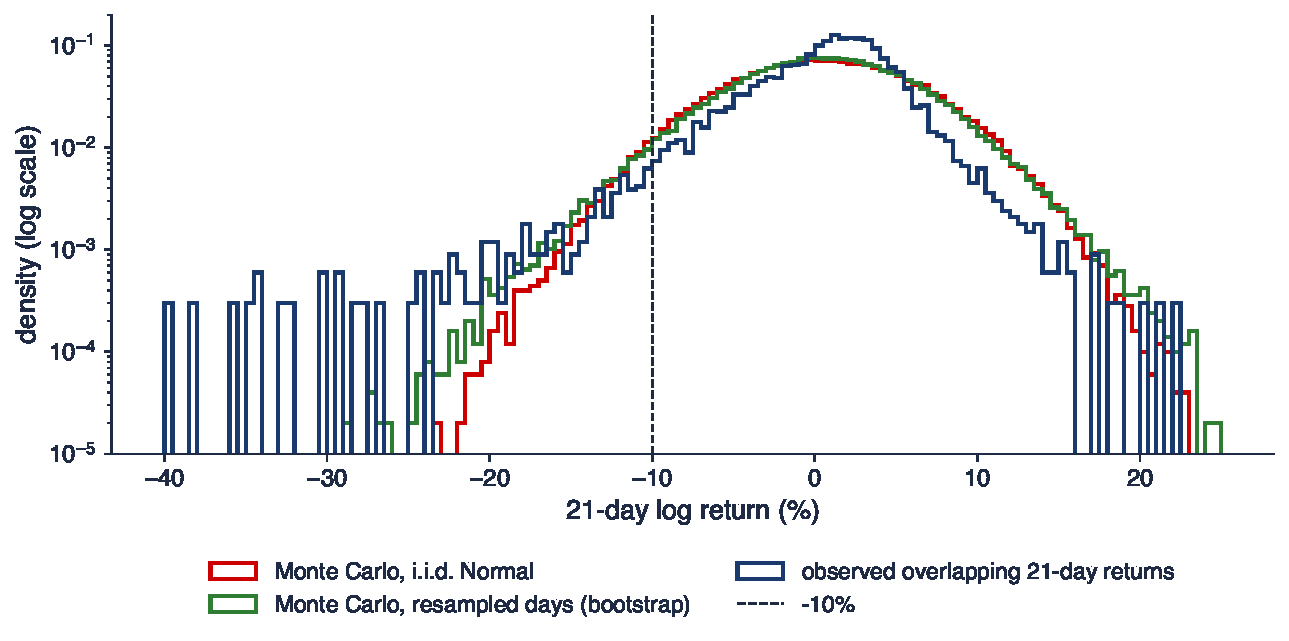
\includegraphics[width=0.96\textwidth,height=0.40\textheight,keepaspectratio]{ch4_sem_b3.pdf}
\end{center}
\vspace{-2mm}
\begin{itemize}
    \item Exact Normal: 2.922\%; Monte Carlo Normal: 2.917\% (s.e. 0.053\%); bootstrap: 3.184\% (s.e. 0.056\%)
    \item Data: 2.67\% of 6\,694 overlapping windows (179 windows, from a few episodes); non-overlapping months: 3.45\% of 319
    \item Interpretation: Monte Carlo vs exact differs by less than one s.e. (simulation error); bootstrap vs Normal differs by about 3.5 s.e. (model error: heavier daily tails); the data are noisy because overlapping windows are dependent
\end{itemize}\sfmquantlet{Ch_04}{SFM_ch4_seminar}
\end{frame}

\begin{frame}{B4: Test a Random Number Generator [Proposed]}
\itemsize{\footnotesize}
\begin{itemize}
\item \textbf{Question}: can a generator pass simple tests and still be unusable?
\item \textbf{Inputs}: RANDU, $x_{k+1} = 65539\,x_k \bmod 2^{31}$, seed 1, 100\,000 numbers; NumPy PCG64 with the same seed; model: B3
\item \textbf{Tasks}
\begin{enumerate}
    \item Compute the mean, the variance and the lag-1 correlation of both sequences and compare with $1/2$, $1/12$ and 0.
    \item Count the distinct values of $9u_k - 6u_{k+1} + u_{k+2}$ for both generators.
    \item Find the period of the LCGs $(a, c, M) = (5, 1, 16)$, $(5, 0, 16)$ and $(4, 1, 16)$ started at 7.
    \item Interpretation: why do one-dimensional tests not detect the flaw of RANDU?
\end{enumerate}
\item \textbf{Report}: a table of six statistics, two counts, three periods, one sentence
\item Notebook: section B4
\end{itemize}
\end{frame}

\ifsolutions
\begin{frame}{B4: Solution [Proposed]}
\itemsize{\footnotesize}
\begin{center}
\footnotesize
\begin{tabular}{lrrrr}
\toprule
Generator & mean & variance & $\rho(1)$ & distinct values \\
\midrule
RANDU & $0.5019$ & $0.0833$ & $0.0008$ & 15 \\
PCG64 & $0.5000$ & $0.0834$ & $0.0030$ & 99\,571 \\
\bottomrule
\end{tabular}
\end{center}
\begin{itemize}
    \item Both pass the moment and lag-1 tests ($1/12 = 0.0833$); RANDU's combination takes only 15 values: its triples lie on 15 planes
    \item Periods: (5, 1, 16): 16; (5, 0, 16): 4; (4, 1, 16): 1
    \item Interpretation: the flaw is in the joint distribution of consecutive numbers; tests of the marginal distribution or of a single lag cannot see it; any 3-dimensional simulation with RANDU is biased
\end{itemize}\sfmquantlet{Ch_04}{SFM_ch4_seminar}
\end{frame}
\fi

\begin{frame}{B5: Is the BET a Geometric Brownian Motion? [Solved]}
\itemsize{\footnotesize}
\begin{itemize}
\item \textbf{Question}: which features of the BET can a GBM with the same drift and volatility reproduce?
\item \textbf{Inputs}: BET closes, 2000--2026; 500 GBM paths of the same length
\item \textbf{Tasks}
\begin{enumerate}
    \item Calibrate GBM: annual log drift and volatility from the daily log returns.
    \item Simulate 500 paths and compute, for each, the excess kurtosis, $\text{Corr}(r_t^2, r_{t-1}^2)$ and the maximum drawdown.
    \item Locate the real values in the simulated distributions (5\% and 95\% quantiles).
    \item Interpretation: which stylised facts does GBM miss, and which risk number is most affected?
\end{enumerate}
\item \textbf{Report}: two parameters, three comparisons, one sentence
\item Notebook: section B5
\end{itemize}
\end{frame}

\begin{frame}{B5: Solution [Solved]}
\itemsize{\scriptsize}
\begin{center}
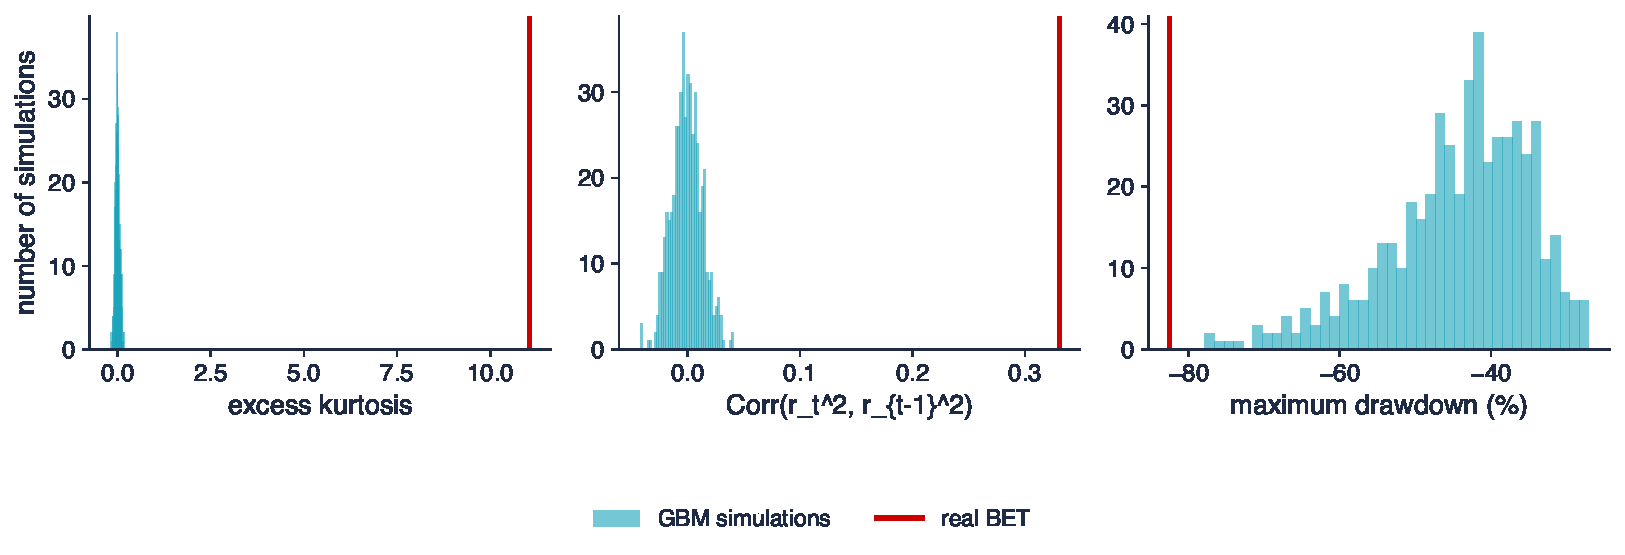
\includegraphics[width=0.96\textwidth,height=0.36\textheight,keepaspectratio]{ch4_sem_b5.pdf}
\end{center}
\vspace{-2mm}
\begin{itemize}
    \item $n = 6\,670$ days; $\sigma = 22.1\%$, log drift 16.0\% a year
    \item Excess kurtosis: real $11.06$, GBM 90\% range $[-0.10, 0.10]$; $\text{Corr}(r_t^2, r_{t-1}^2)$: real $0.330$, GBM $[-0.022, 0.022]$
    \item Maximum drawdown: real $-82.5\%$, GBM median $-42.7\%$, range $[-62.8\%, -31.4\%]$
    \item Interpretation: GBM misses heavy tails and volatility clustering completely; the 2008 crash makes the real drawdown deeper than every simulated path, so a GBM-based risk limit would have been far too loose
\end{itemize}\sfmquantlet{Ch_04}{SFM_ch4_seminar}
\end{frame}

\begin{frame}{B6: Does Variance Grow Linearly with the Horizon? [Proposed]}
\itemsize{\footnotesize}
\begin{itemize}
\item \textbf{Question}: does $\text{Var}(h\text{-day return}) = h\,\text{Var}(1\text{-day return})$ hold, as a random walk with i.i.d. increments predicts?
\item \textbf{Inputs}: S\&P 500, BET, Bitcoin daily log returns; non-overlapping blocks of $h = 5, 21, 63$ days; model: B5
\item \textbf{Tasks}
\begin{enumerate}
    \item Compute the ratio $\text{Var}(h\text{-day})/(h\,\text{Var}(1\text{-day}))$ for each series and horizon.
    \item Use the approximate standard error $\sqrt{2/(m - 1)}$ of a variance ratio with $m$ blocks to judge the distance from 1.
    \item Interpretation: what does a ratio above 1 or below 1 say about the autocorrelation of returns?
\end{enumerate}
\item \textbf{Report}: a $3 \times 3$ table and two sentences
\item Notebook: section B6
\end{itemize}
\end{frame}

\ifsolutions
\begin{frame}{B6: Solution [Proposed]}
\itemsize{\footnotesize}
\begin{center}
\footnotesize
\begin{tabular}{lrrr}
\toprule
Series & $h = 5$ & $h = 21$ & $h = 63$ \\
\midrule
S\&P 500 & $0.84$ & $0.80$ & $0.66$ \\
BET & $1.15$ & $1.37$ & $1.68$ \\
Bitcoin & $0.96$ & $1.16$ & $1.28$ \\
approx. s.e. (S\&P 500) & $0.04$ & $0.08$ & $0.14$ \\
\bottomrule
\end{tabular}
\end{center}
\begin{itemize}
    \item S\&P 500 below 1 (mean reversion over weeks, mostly from crisis rebounds); BET above 1 and growing (positive autocorrelation, thin trading); Bitcoin within about two s.e. of 1
    \item Interpretation: $\text{Var}(\sum r) = h\sigma^2 + 2\sum_{i<j}\text{Cov}(r_i, r_j)$; positive autocorrelations push the ratio above 1, negative ones below 1
    \item This is the variance-ratio test of Chapter 7, with its proper standard errors
\end{itemize}\sfmquantlet{Ch_04}{SFM_ch4_seminar}
\end{frame}
\fi


%=============================================================================
\section{Part C: Open Questions and AI Critique}
%=============================================================================

\begin{frame}{C1: How Often Is There a Bad Year? [Proposed]}
\itemsize{\footnotesize}
\begin{itemize}
\item \textbf{Question}: does GBM give the right probability of a drawdown beyond 20\% (or 40\%) within one calendar year?
\item \textbf{Inputs}: S\&P 500, DAX, BET, Bitcoin, complete calendar years 2000--2025 (Bitcoin 2015--2025); models: B3, B5
\item \textbf{Tasks}
\begin{enumerate}
    \item Compute the maximum drawdown within each calendar year and the share of years beyond 20\% and beyond 40\%.
    \item Simulate 10\,000 one-year paths under GBM and under the i.i.d. bootstrap of the daily returns and compute the same two probabilities.
    \item Compare data and models with a binomial test.
    \item Propose one model that could reproduce both numbers.
    \item Interpretation: what does the gap between the bootstrap and the data say about volatility clustering?
\end{enumerate}
\item \textbf{Report}: a table, two binomial $p$-values, a short project plan
\item Notebook: section C1
\end{itemize}
\end{frame}

\ifsolutions
\begin{frame}{C1: Reference Analysis [Proposed]}
\itemsize{\footnotesize}
\begin{center}
\footnotesize
\begin{tabular}{lrrrrrrr}
\toprule
Series & years & data 20\% & GBM & boot. & data 40\% & GBM & boot. \\
\midrule
S\&P 500 & 26 & 23.1 & 33.1 & 31.4 & 3.8 & 0.5 & 0.6 \\
DAX & 26 & 42.3 & 50.2 & 47.5 & 11.5 & 2.2 & 2.4 \\
BET & 26 & 46.2 & 33.5 & 31.8 & 3.8 & 0.7 & 0.8 \\
Bitcoin & 11 & 100.0 & 99.8 & 99.4 & 54.5 & 62.8 & 60.9 \\
\bottomrule
\end{tabular}
\end{center}
\begin{itemize}
    \item 20\%: GBM and bootstrap agree with each other; the S\&P 500 had fewer bad years than both, the BET more
    \item 40\%: both models give well under 3\% for the indices, but 2008 (and for the DAX 2001--2002) happened: deep drawdowns need clustered volatility, not only heavy tails
    \item Project directions: GARCH(1,1) and regime-switching simulations, block bootstrap, more indices, a formal test on 26 years
\end{itemize}\sfmquantlet{Ch_04}{SFM_ch4_seminar}
\end{frame}
\fi

\begin{frame}{C2: Audit an AI Answer [Proposed]}
\itemsize{\scriptsize}
\begin{itemize}
    \item A student asked an AI assistant to ``summarise the probability facts about the S\&P 500 for a risk report''. The answer:
    \item \aiprompt{(a) Corr(r\_t, r\_\{t-1\}) = -0.099, so daily returns are independent and tomorrow's variance cannot be predicted.}
    \item \aiprompt{(b) The log price is a random walk, so its variance is the same at every date and the process is stationary.}
    \item \aiprompt{(c) Under GBM with mu = 8\% and sigma = 19\%, the median value of 100 after 10 years is 100 exp(0.8) = 222.6.}
    \item \aiprompt{(d) A Monte Carlo probability of about 3\% from 10,000 paths has a standard error of about 0.0017.}
    \item \aiprompt{(e) A 50/50 portfolio of S\&P 500 and DAX has daily volatility sqrt(0.25 x 1.22\textasciicircum 2 + 0.25 x 1.43\textasciicircum 2) = 0.94\%.}
    \item Tasks
    \begin{itemize}
        \item 1. For each statement, say whether it is correct; if not, give the correct statement and the correct number from the notebook (section C2).
        \item 2. Report: a list of five verdicts with one line of justification each.
    \end{itemize}
\end{itemize}
\end{frame}

\ifsolutions
\begin{frame}{C2: Solution [Proposed]}
\itemsize{\footnotesize}
\begin{itemize}
    \item (a) Wrong: uncorrelated is not independent; $\text{Corr}(r_t^2, r_{t-1}^2) = 0.31$ and the conditional s.d. after the most turbulent days is 1.88 times that after the calmest
    \item (b) Wrong: $\text{Var}(S_t) = t\sigma^2$ grows with $t$; a random walk is not stationary (its increments are)
    \item (c) Wrong: $100e^{\mu T} = 222.6$ is the mean; the median is $100e^{(\mu - \sigma^2/2)T} = 185.8$
    \item (d) Correct: $\sqrt{0.03 \times 0.97/10\,000} = 0.0017$; the error falls like $1/\sqrt{N}$, not $1/N$
    \item (e) Wrong: the covariance term is missing; with $\rho = 0.60$ the volatility is $1.19\%$, not $0.94\%$: the AI understates the risk
\end{itemize}\sfmquantlet{Ch_04}{SFM_ch4_seminar}
\end{frame}
\fi


%=============================================================================
\section{Wrap-Up}
%=============================================================================

\begin{frame}{What You Should Take from Today}
\itemsize{\small}
\begin{itemize}
    \item Zero correlation does not mean independence: check squares or absolute values too
    \item The conditional variance of returns moves with yesterday's news; the conditional mean hardly moves
    \item Mixtures of Normal regimes give heavy tails
    \item Monte Carlo: report the standard error; separate simulation error from model error
    \item GBM reproduces the path of an index roughly, but not its tails, clusters or deepest drawdowns
    \item An AI answer is a draft: check every definition, model and number
\end{itemize}
\end{frame}

\begin{frame}{After the Seminar}
\itemsize{\small}
\begin{itemize}
    \item Lecture 4 develops each topic of today: distributions, dependence, conditioning, Monte Carlo, binomial trees, random walks, Wiener process and GBM
    \item Try the [Proposed] tasks in the notebook; the solutions are discussed in class
    \item C1 can grow into a team project: GARCH and regime-switching simulations, block bootstrap, more indices
    \item Reading: \refFHH, Ch.~3--5; exercises with solutions: \refFHHex
\end{itemize}
\end{frame}


%=============================================================================
\section{References}
%=============================================================================

\begin{frame}{References}
\itemsize{\tiny}
\begin{itemize}
    \item Borak, S., Härdle, W.K., López-Cabrera, B. (2013). \href{https://doi.org/10.1007/978-3-642-33929-5}{\textit{Statistics of Financial Markets: Exercises and Solutions}}, 2nd ed. Springer.
    \item Cox, J.C., Ross, S.A., Rubinstein, M. (1979). \href{https://doi.org/10.1016/0304-405X(79)90015-1}{Option pricing: a simplified approach}. \textit{Journal of Financial Economics}, 7(3), 229--263.
    \item Franke, J., Härdle, W.K., Hafner, C.M. (2019). \href{https://doi.org/10.1007/978-3-030-13751-9}{\textit{Statistics of Financial Markets: An Introduction}}, 5th ed. Springer.
    \item Glasserman, P. (2003). \href{https://doi.org/10.1007/978-0-387-21617-1}{\textit{Monte Carlo Methods in Financial Engineering}}. Springer.
    \item Marsaglia, G. (1968). \href{https://doi.org/10.1073/pnas.61.1.25}{Random numbers fall mainly in the planes}. \textit{Proceedings of the National Academy of Sciences}, 61(1), 25--28.
\end{itemize}
\end{frame}

\end{document}
